    % Autor: Tomáš Daniel           <xdanie14@stud.fit.vutbr.cz>
    % Autor: Martin Slezák          <xsleza26@stud.fit.vutbr.cz>
    % Autor: Jakub Antonín Štigler  <xstigl00@stud.fit.vutbr.cz>
    % Autor: Milan Vrbas            <xvrbas01@stud.fit.vutbr.cz>

    \documentclass[a4paper, 12pt]{article} % definice třídy dokumentu a nastavení vlastností

    % balíčky
    \usepackage[utf8]{inputenc} % nastavení kódování
    \usepackage{times} % font
    \usepackage[czech]{babel} % čeština
    \usepackage[IL2]{fontenc} % nastavení kódování fontů
    \usepackage[left=2cm, text={17cm, 24cm}, top=3cm]{geometry} % nastavení rozměrů stránky
    \usepackage{graphics} % obrázky
    \usepackage[unicode]{hyperref} % odkazy
    \usepackage{pdflscape} % otočení stránky
    \usepackage{fancyhdr} % zkrášlení stránky
    \usepackage{enumitem} % nastavení seznamů
    \usepackage{xparse} % pro barvy
    \usepackage{tabularx} % lepší tabulky
    \usepackage{array} % lepší tabulky
    \usepackage[table]{xcolor} % barvy tabulek
    \usepackage{float}
    \usepackage{csquotes}

    
 

    %%%%%%%%%%%%%%%%%%%%%%%%%%%%%%% Makra a přizpůsobení dokumentu %%%%%%%%%%%%%%%%%%%%%%%%%%%%%%%%
    \newcolumntype{Y}{>{\centering\arraybackslash}X}
    \NewDocumentCommand{\orange}{m}{\textcolor{orange}{\texttt{#1}}} % oranžová barva textu
    \NewDocumentCommand{\blue}{m}{\textcolor{blue}{\texttt{#1}}} % modrá barva textu
    \renewcommand{\arraystretch}{1.2} % Větší mezery v tabulce

    \pagestyle{fancy}
    \fancyhf{}
    \fancyfoot[C]{\thepage} % čára na začátku stránky

    \def\fillandplacepagenumber{%
        \par\pagestyle{empty}%
        \vbox to 0pt{\vss}\vfill
        \vbox to 0pt{\baselineskip0pt
            \hbox to\linewidth{\hss}%
            \baselineskip\footskip
            \hbox to\linewidth{%
                \hfil\thepage\hfil}\vss}} % číslo ležaté stránky dolů
    %%%%%%%%%%%%%%%%%%%%%%%%%%%%%%% Makra a přizpůsobení dokumentu %%%%%%%%%%%%%%%%%%%%%%%%%%%%%%%%
    \begin{document}
    %%%%%%%%%%%%%%%%%%%%%%%%%%%%%%%%%%%%%%%% Úvodní strana %%%%%%%%%%%%%%%%%%%%%%%%%%%%%%%%%%%%%%%%
        \begin{titlepage}
            \begin{center}
        \scalebox{0.15}{
\includegraphics{pictures/FIT_logo.png}} \\
                \vspace{\stretch{0.382}}
                \Huge{Projektová dokumentace} \\
                \Large{\textbf{Implementace překladače imperativního jazyka IFJ23}} \\
                \large{Tým xdanie14, varianta vv-BVS}
                \vspace{\stretch{0.618}}
            \end{center}

        {\large \today \hfill
        \large
        \begin{tabular}{l l l}
        \textbf{Tomáš Daniel} & \quad \textbf{xdanie14} & \quad X\,\% \\
        Martin Slezák         & \quad xsleza26          & \quad X\,\% \\
        Jakub Antonín Štigler & \quad xstigl00          & \quad X\,\% \\
        Milan Vrbas           & \quad xvrbas01          & \quad X\,\% \\
        \end{tabular}
        }
    \end{titlepage}
    %%%%%%%%%%%%%%%%%%%%%%%%%%%%%%%%%%%%%%%% Úvodní strana %%%%%%%%%%%%%%%%%%%%%%%%%%%%%%%%%%%%%%%%

    %%%%%%%%%%%%%%%%%%%%%%%%%%%%%%%%%%%%%%%%%%%% Obsah %%%%%%%%%%%%%%%%%%%%%%%%%%%%%%%%%%%%%%%%%%%%
    \tableofcontents
    \thispagestyle{empty}
    \newpage
    %%%%%%%%%%%%%%%%%%%%%%%%%%%%%%%%%%%%%%%%%%%% Obsah %%%%%%%%%%%%%%%%%%%%%%%%%%%%%%%%%%%%%%%%%%%%   

    %%%%%%%%%%%%%%%%%%%%%%%%%%%%%%%%%%%%%%%%%%%% Úvod %%%%%%%%%%%%%%%%%%%%%%%%%%%%%%%%%%%%%%%%%%%%% 
    \setcounter{page}{1}
    \section{Úvod}
    Tato dokumentace slouží k popisu implementace a vývoje \textbf{překladače pro jazyk IFJ23}, 
    který je podmnožinou jazyka \textbf{Swift 5} od společnosti Apple. Program má za úkol načíst 
    kód v tomto jazyku a přeložit ho do cílového jazyka \textbf{IFJcode23}. Vybrali jsme si variantu 
    zadání \textbf{vv-BVS}, podle které jsme pomocí \textbf{výškově vyváženého binárního 
    vyhledávacího stromu} implementovali \textbf{tabulku symbolů}.
    %%%%%%%%%%%%%%%%%%%%%%%%%%%%%%%%%%%%%%%%%%%% Úvod %%%%%%%%%%%%%%%%%%%%%%%%%%%%%%%%%%%%%%%%%%%%% 

    %%%%%%%%%%%%%%%%%%%%%%%%%%%%%%%%%%%%%% Části překladače %%%%%%%%%%%%%%%%%%%%%%%%%%%%%%%%%%%%%%% 
    \section{Jednotlivé části překladače}
    Realizovaný překladač se dá rozdělit na následující dílní moduly:
    \begin{itemize}[noitemsep]
        \item \hyperref[lexer]{\textbf{Scanner}} - lexikální analyzátor
        \item \textbf{Parser}
            \begin{itemize}
                \item \hyperref[syntactics]{Syntaktický analyzátor}
                \item \hyperref[semantics]{Sémantický analyzátor}
            \end{itemize}
        \item \hyperref[codegen]{\textbf{Codegen}} - Genérátor cílového kódu
    \end{itemize}
    Samotný překlad nejprve provede lexikální analýzu, následuje syntaktický 
    analyzátor spolu se sémantickou analýzou a poté se přistoupí k generování 
    cílového kódu. 
    %%%%%%%%%%%%%%%%%%%%%%%%%%%%%%%%%%%%%% Části překladače %%%%%%%%%%%%%%%%%%%%%%%%%%%%%%%%%%%%%%% 

    %%%%%%%%%%%%%%%%%%%%%%%%%%%%%%%%%%%%% Lexikální analýza %%%%%%%%%%%%%%%%%%%%%%%%%%%%%%%%%%%%%%% 
    \section{Návrh a implementace} \label{lexer}
        \subsection{Lexikální analýza}
            Jako první část projektu, kterou jsme implementovali byla lexikální analýza, kterou
            lze najít v modulu \textit{lexer.c}. Ta se
            stará o načítání znaků neboli lexémů ze standartního vstupu a rozdělování vstupních dat na 
            jednotlivé tokeny, u nichž následně určuje jejich typ a posílá 
            je k syntaktické a sémantické analýze k 
            dalšímu zpracování. 

            Lexikální analýza využívá koncept \hyperref[kodiagram]{\textbf{konečného automatu}} pro 
            identifikaci a zpracování tokenů ve vstupním kódu. Tento přístup umožňuje systematicky 
            analyzovat postupně načtené znaky a identifikovat je jako jednotlivé tokeny na základě 
            definovaných pravidel a přechodů mezi stavy automatu. Tímto způsobem je struktura 
            vstupního kódu efektivně analyzována a převedena do podoby tokenů pro další zpracování. 

            Funkce \textit{lex\_next()} zajišťuje většinu vnitřní logiky scanneru tím, že načte 
            token a uloží ho do struktury \textit{Lexer}, která obsahuje důležité informace o každém 
            předaném tokenu. V případě, že ve zdrojovém souboru narazí na neplatný token či neplatnou
            posloupnost znaků, překladač skončí s návratovou hodnotou, která odpovídá konkrétnímu 
            příznaku lexikální chyby. 


            \newpage
            \subsubsection{Diagram konečného automatu} \label{kodiagram}
                \begin{figure}[H]
                    \centering
                    \scalebox{0.081}{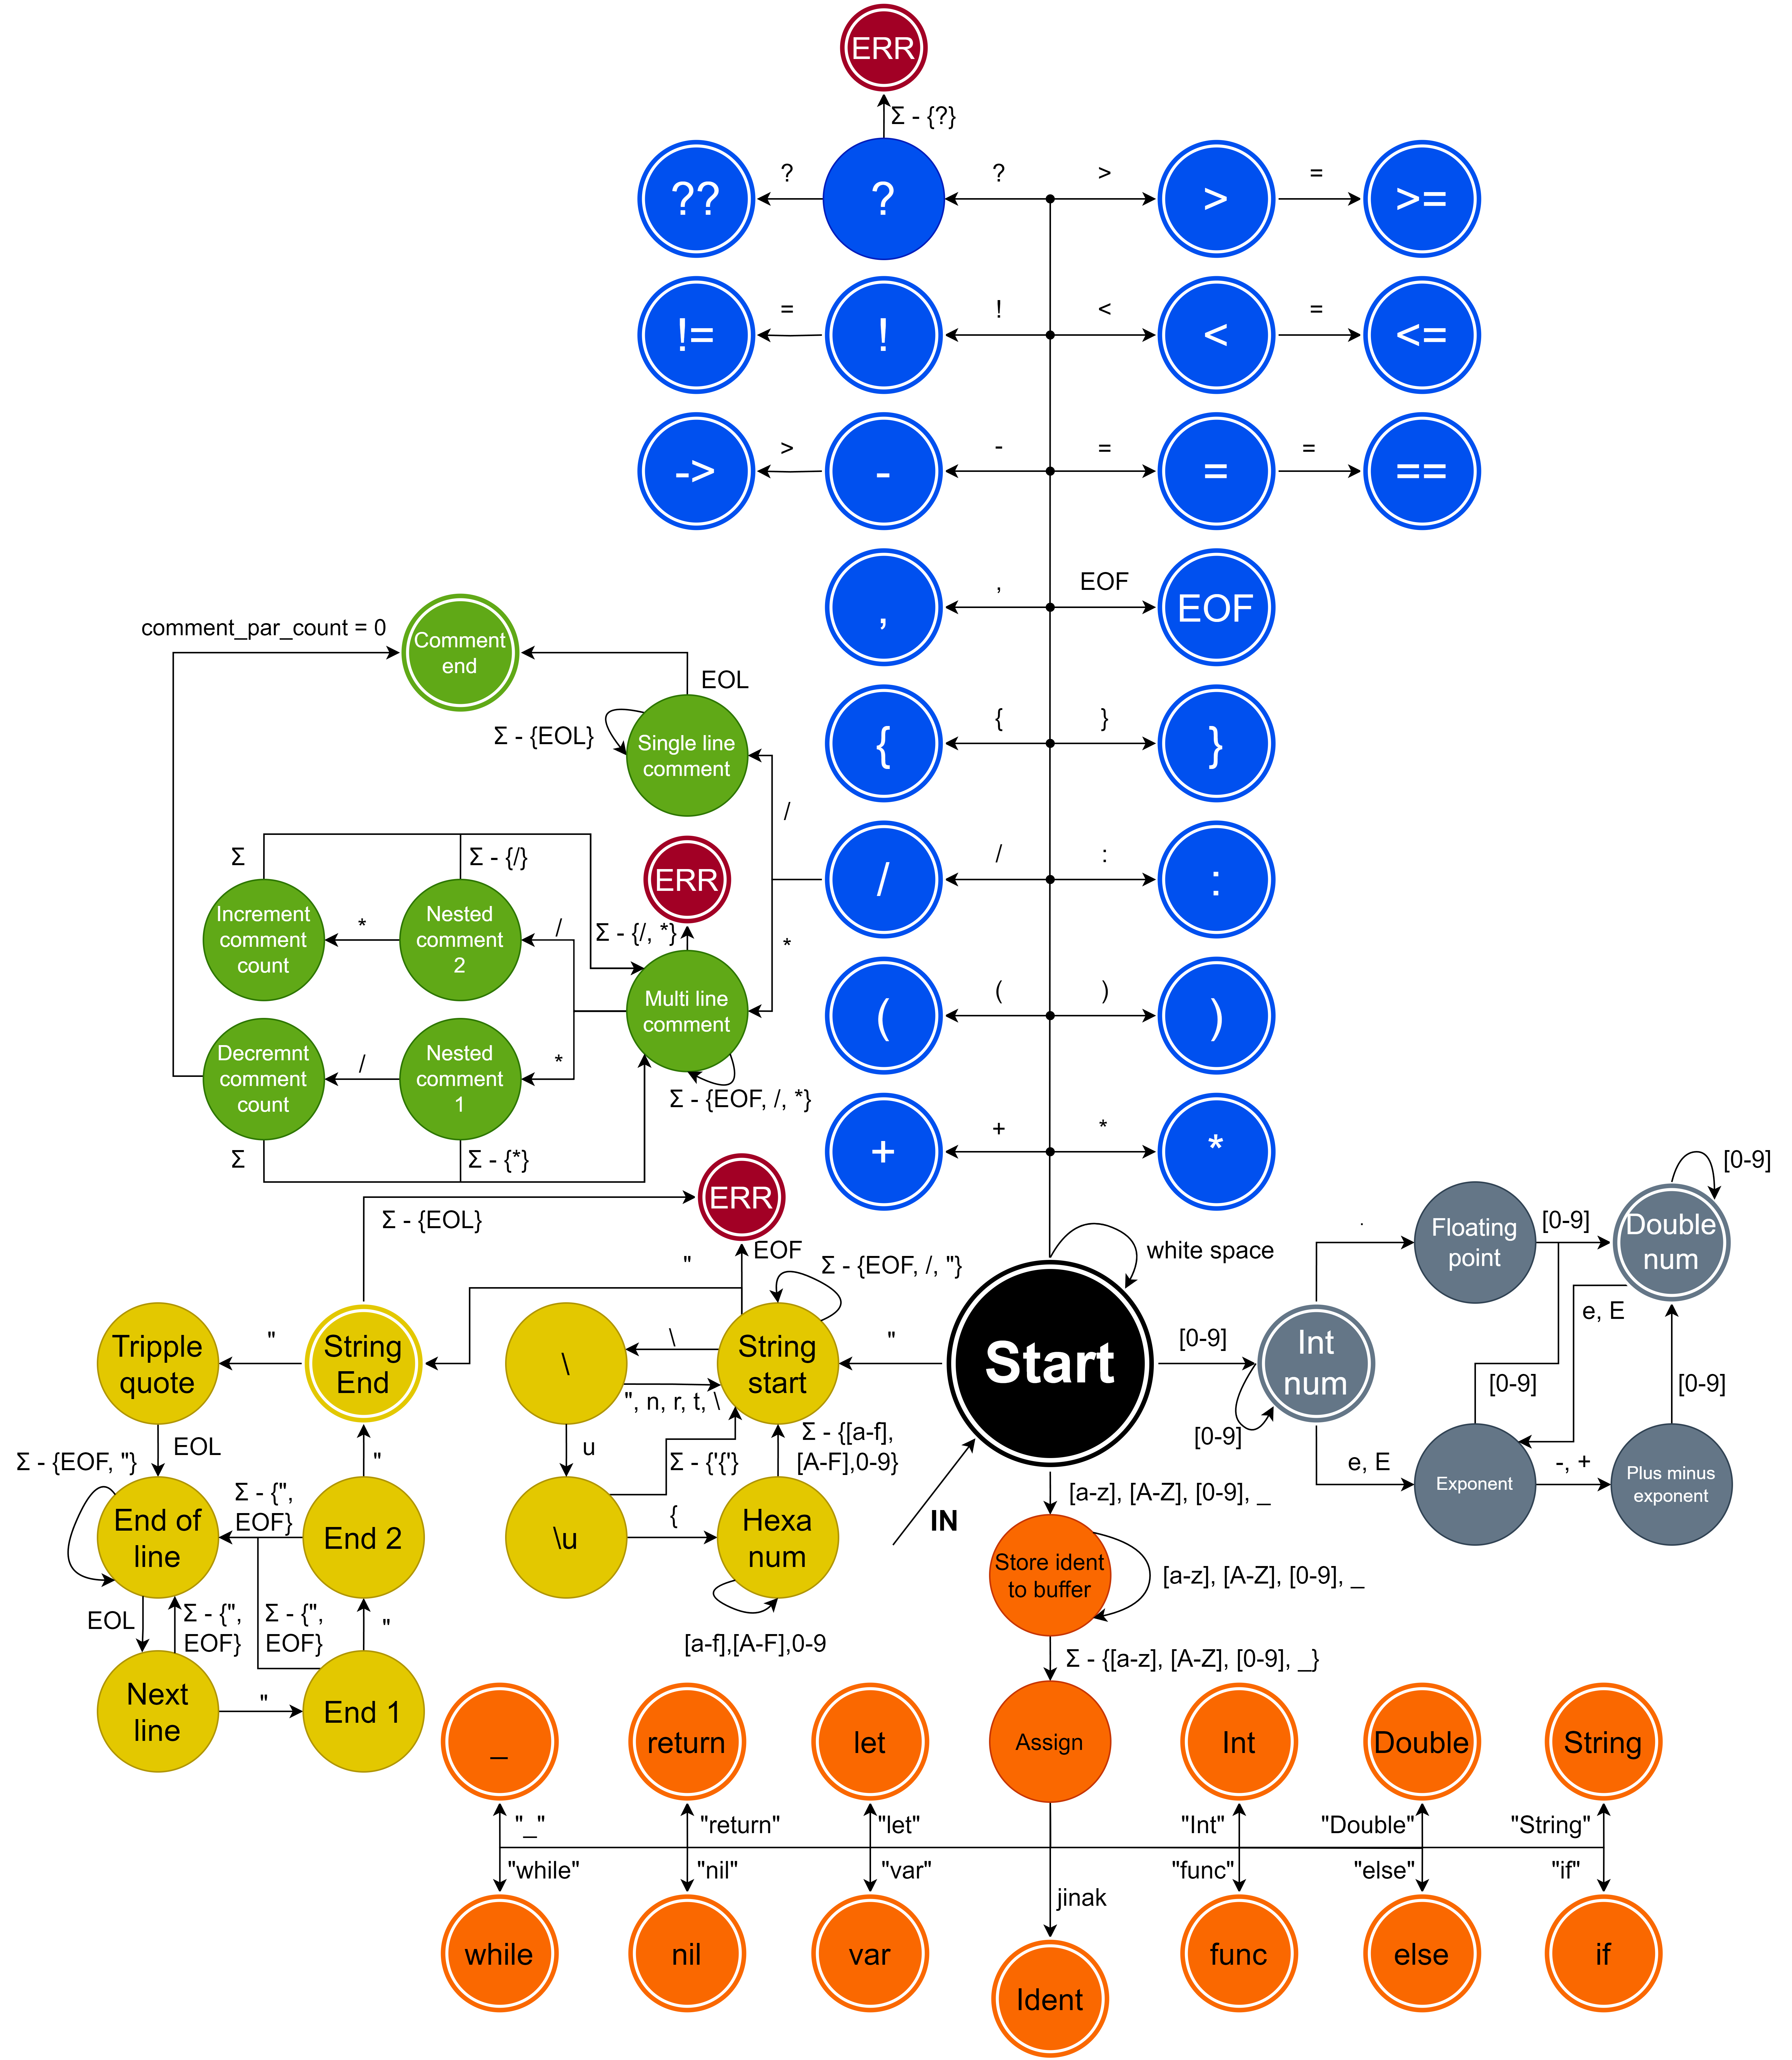
\includegraphics{pictures/KO.png}}
                    \caption{Diagram zobrazující konečný automat}
                \end{figure}

                \rule{5cm}{0.4pt} \\
                {\footnotesize Poznámka: pokud automat nemá možnost přejít do dalšího stavu z 
                nekoncového stavu, je to automaticky bráno jako chyba. (pro zjednodušení návrhu
                automatu)}
            \newpage

    %%%%%%%%%%%%%%%%%%%%%%%%%%%%%%%%%%%%% Lexikální analýza %%%%%%%%%%%%%%%%%%%%%%%%%%%%%%%%%%%%%%% 

    %%%%%%%%%%%%%%%%%%%%%%%%%%%%%%%%%%%% Syntaktická analýza %%%%%%%%%%%%%%%%%%%%%%%%%%%%%%%%%%%%%% 
        \subsection{Syntaktická analýza} \label{syntactics}
            \subsubsection{Rekurzivní sestup}
                Implementace syntaktické analýzy se nachází v souboru \textbf{parser.c}, který se
                zaobírá aplikací metody shora dolů, respektive \textbf{rekurzivního sestupu}, který
                je složen z \hyperref[llgramatika]{\textbf{LL--gramatiky}} a 
                \hyperref[lltabulka]{\textbf{LL--tabulky}}. Parser si za svůj vstup bere jednotlivé 
                tokeny z lexikální analýzy a následně nalpní tabulku symbolů v podobě výškově 
                vyváženého binárního vyhledávacího stromu (vv-BVS). Pro většinu neterminálů z 
                LL-gramatiky je sestavena funkce, která následně volá další funkce na základě 
                předcházejícího tokenu. Tyto tokeny se získávají pomocí funkce \textit{lex\_next()}.
            %%%%%%%%%%%%%%%%%%%%%%% LL-gramatika %%%%%%%%%%%%%%%%%%%%%%%
            {\fontsize{10.1}{13.4}\selectfont
            \subsubsection*{LL--gramatika}\label{llgramatika}
            \begin{enumerate}[noitemsep]
                \item \texttt{MAIN -> \orange{"EOF"}}
                \item \texttt{MAIN -> STATEMENT MAIN}
                \item \texttt{{MAIN -> \orange{"func"'~ident~"("} PARAMS \orange{")"}
                RETVAL \orange{"\{"}} STATEMENT \orange{"\}"} MAIN }
                \item \texttt{STATEMENT -> \blue{$\epsilon$}}
                \item \texttt{PARAMS -> \blue{$\epsilon$}}
                \item \texttt{PARAMS -> \orange{name~ident~":"} TYPE PARAMS\_NEXT}
                \item \texttt{TYPE -> \orange{"Int"} Q\_MARK}
                \item \texttt{TYPE -> \orange{"Double"} Q\_MARK}
                \item \texttt{TYPE -> \orange{"String"} Q\_MARK}
                \item \texttt{Q\_MARK -> \blue{$\epsilon$}}
                \item \texttt{Q\_MARK -> \orange{"?"}}
                \item \texttt{PARAMS\_NEXT -> \blue{$\epsilon$}}
                \item \texttt{PARAMS\_NEXT -> \orange{","} PARAMS}
                \item \texttt{RETVAL -> \blue{$\epsilon$}}
                \item \texttt{RETVAL -> \orange{"->"} TYPE}
                \item \texttt{STATEMENT -> VAR RIGHTSIDE STATEMENT}
                \item \texttt{VAR -> \orange{"let"~ident~":"} TYPE}
                \item \texttt{VAR -> \orange{"var"~ident~":"} TYPE}
                \item \texttt{RIGHTSIDE -> \blue{$\epsilon$}}
                \item \texttt{RIGHTSIDE -> \orange{"$=$"} EXPR}
                \item \texttt{EXPR -> \orange{"Do~it~using~precedence~table"}}
                \item \texttt{STATEMENT -> \orange{ident~"$=$"} EXPR STATEMENT}
                \item \texttt{{STATEMENT -> \orange{"$=$"} COND \orange{"\{"}} 
                STATEMENT \orange{"\}"} ELSESTAT}
                \item \texttt{COND -> EXPR}
                \item \texttt{COND -> \orange{"("~"let"~ident~")"}}
                \item \texttt{COND -> \orange{"let"~ident}}
                \item \texttt{ELSESTAT -> STATEMENT}
                \item \texttt{{ELSESTAT -> \orange{"else"~"\{"}} STATEMENT 
                \orange{"\}"}STATEMENT}
                \item \texttt{{WHILESTAT -> \orange{"while"} COND \orange{"\{"}} 
                STATEMENT \orange{"\}"} STATEMENT}
                \item \texttt{FUNCCALL -> LEFTSIDE \orange{ident~"("} FUNCPARAMS 
                \orange{")"} STATEMENT}
                \item \texttt{LEFTSIDE -> \blue{$\epsilon$}}
                \item \texttt{LEFTSIDE -> VAR \orange{"$=$"}}
                \item \texttt{FUNCPARAMS -> \blue{$\epsilon$}}
                \item \texttt{FUNCPARAMS -> \orange{ident~":"~name} FUNCPARAMS\_NEXT}
                \item \texttt{FUNCPARAMS -> \orange{name} FUNCPARAMS\_NEXT}
                \item \texttt{FUNCPARAMS\_NEXT -> \blue{$\epsilon$}}
                \item \texttt{FUNCPARAMS\_NEXT -> \orange{","} FUNCPARAMS}
                \item \texttt{STATEMENT -> \orange{"return"} VALUE STATEMENT}
                \item \texttt{VALUE -> EXPR}
            \end{enumerate}}
            %%%%%%%%%%%%%%%%%%%%%%% LL-gramatika %%%%%%%%%%%%%%%%%%%%%%%

            %%%%%%%%%%%%%%%%%%%%%%%% LL-tabulka %%%%%%%%%%%%%%%%%%%%%%%%
            \newpage
            \begin{landscape}
                \subsubsection*{LL-tabulka}\label{lltabulka}
                \thispagestyle{empty}
                \begin{figure}[htbp]
                    \centering
                    \scalebox{0.566}{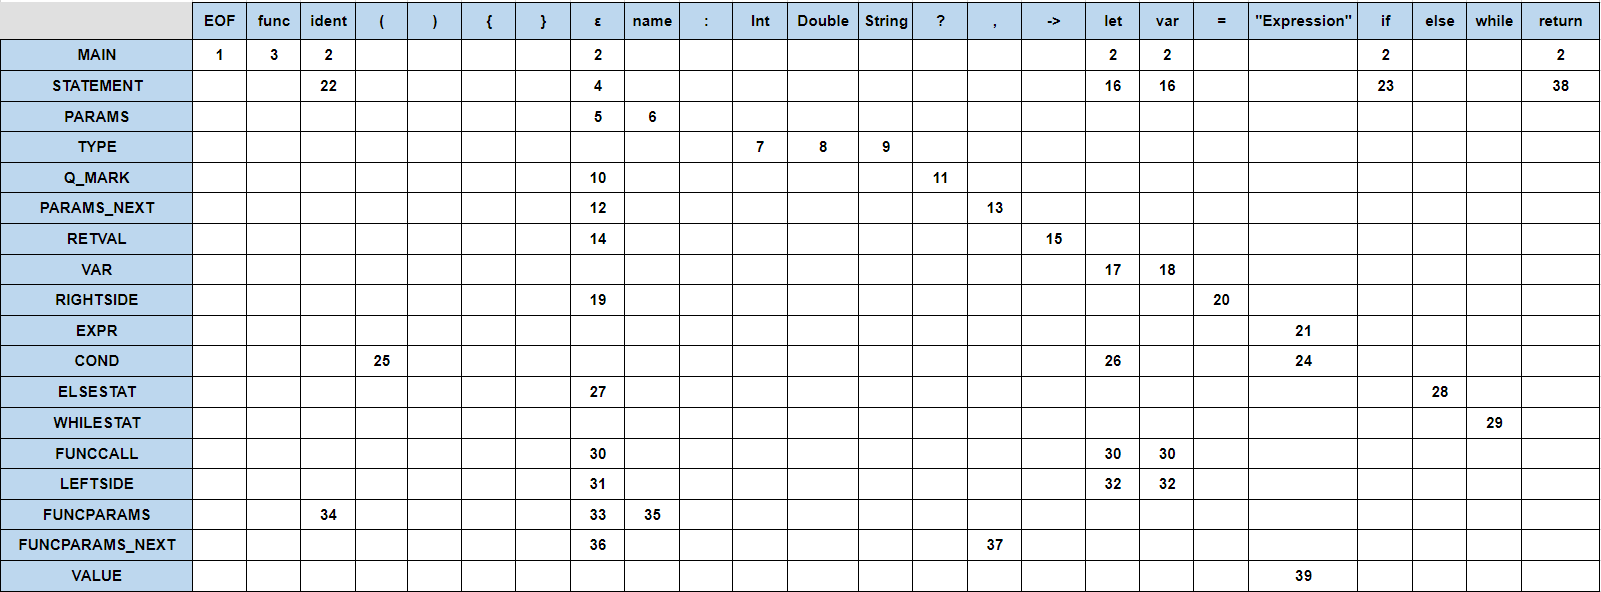
\includegraphics{pictures/LL_tabulka.png}}
                    \caption{Tabulka zobrazující LL-tabulku}
                \end{figure}
                \fillandplacepagenumber
            \end{landscape}
            \newpage
            %%%%%%%%%%%%%%%%%%%%%%%% LL-tabulka %%%%%%%%%%%%%%%%%%%%%%%%

            %%%%%%%%%%%%%%%%%%%%%%% PSA-tabulka %%%%%%%%%%%%%%%%%%%%%%%%
            \subsubsection{Precedenční syntaktická analýza}
                Precedenční syntaktická analýza neboli PSA se stará o syntaktickou analýzu metodou
                zdola-nahoru pomocí \hyperref[prectabulka]{\textbf{precedenční tabulky}}. Na základě
                žádosti PSA pošle lexikální analyzátor token, který se poté zpracuje s nejvyšším tokenem
                na zásobníku a funkce \textit{prec\_table} na základě níže uvedených pravidel vrací to,
                které se má na daný výraz aplikovat. Precedenční syntaktická analýza končí v moment, kdy 
                přijde prázdné pravidlo a zároveň je zásobník (\textit{stack}) prázdný. Následně skončí 
                úspěšně a vrací poslední načtený znak. V opačném případě končí neúspěšně.
            \begin{table}[ht]
                    \centering 
                    \small
                    \begin{tabularx}{\textwidth}{|*{18}{Y|}}
                        \hline
                        \cellcolor{black!80}&  \cellcolor{blue!60}\textbf{$\pi$} &\cellcolor{blue!60} \textbf{*} &\cellcolor{blue!60} \textbf{/} &\cellcolor{blue!60} \textbf{+} &\cellcolor{blue!60} \textbf{-} &\cellcolor{blue!60} \textbf{==} & \cellcolor{blue!60}\textbf{!=} & \cellcolor{blue!60}\textbf{{\textless}} & \cellcolor{blue!60}\textbf{{\textgreater}} & \cellcolor{blue!60}\textbf{{\textless}=} & \cellcolor{blue!60}\textbf{{\textgreater}=} & \cellcolor{blue!60}\textbf{??} & \cellcolor{blue!60}\textbf{=} & \cellcolor{blue!60}\textbf{(} & \cellcolor{blue!60}\textbf{)} & \cellcolor{blue!60}\textbf{$t$} & \cellcolor{blue!60}\textbf{\$} \\
                        \hline
                        \cellcolor{blue!60}\textbf{$\pi$} & \cellcolor{green!75}{\textgreater} & \cellcolor{green!75}{\textgreater} & \cellcolor{green!75}{\textgreater} & \cellcolor{green!75}{\textgreater} & \cellcolor{green!75}{\textgreater} & \cellcolor{green!75}{\textgreater}& \cellcolor{green!75}{\textgreater} & \cellcolor{green!75}{\textgreater}& \cellcolor{green!75}{\textgreater}& \cellcolor{green!75}{\textgreater}& \cellcolor{green!75}{\textgreater}& \cellcolor{green!75}{\textgreater}& \cellcolor{red!60}! & \cellcolor{purple!85}c & \cellcolor{green!75}{\textgreater} & \cellcolor{black!50}{.} & \cellcolor{black!50}{.} \\
                        \hline
                        \cellcolor{blue!60}\textbf{*} & \cellcolor{red!60}!& \cellcolor{green!75}{\textgreater}& \cellcolor{green!75}{\textgreater}& \cellcolor{gray!75}x& \cellcolor{gray!75}x& \cellcolor{green!75}{\textgreater}& \cellcolor{green!75}{\textgreater}& \cellcolor{green!75}{\textgreater}& \cellcolor{green!75}{\textgreater}& \cellcolor{green!75}{\textgreater}& \cellcolor{green!75}{\textgreater}& \cellcolor{green!75}{\textgreater}& \cellcolor{red!60}!& \cellcolor{yellow!75}{\textless}& \cellcolor{green!75}{\textgreater}& \cellcolor{yellow!75}{\textless}& \cellcolor{black!50}{.}\\
                        \hline
                        \cellcolor{blue!60}\textbf{/} &\cellcolor{red!60}! & \cellcolor{green!75}{\textgreater}& \cellcolor{green!75}{\textgreater}& \cellcolor{gray!75}x& \cellcolor{gray!75}x& \cellcolor{green!75}{\textgreater}& \cellcolor{green!75}{\textgreater}& \cellcolor{green!75}{\textgreater}& \cellcolor{green!75}{\textgreater}& \cellcolor{green!75}{\textgreater}& \cellcolor{green!75}{\textgreater}& \cellcolor{green!75}{\textgreater}& \cellcolor{red!60}!& \cellcolor{yellow!75}{\textless}& \cellcolor{green!75}{\textgreater}& \cellcolor{yellow!75}{\textless}& \cellcolor{black!50}{.}\\
                        \hline
                        \cellcolor{blue!60}\textbf{+} & \cellcolor{red!60}! & \cellcolor{gray!75}0& \cellcolor{gray!75}0&\cellcolor{green!75}{\textgreater}& \cellcolor{green!75}{\textgreater}&\cellcolor{green!75}{\textgreater}& \cellcolor{green!75}{\textgreater}& \cellcolor{green!75}{\textgreater}& \cellcolor{green!75}{\textgreater}& \cellcolor{green!75}{\textgreater}& \cellcolor{green!75}{\textgreater}& \cellcolor{green!75}{\textgreater}& \cellcolor{red!60}!& \cellcolor{yellow!75}{\textless}& \cellcolor{green!75}{\textgreater}& \cellcolor{yellow!75}{\textless}& \cellcolor{black!50}{.}\\
                        \hline
                        \cellcolor{blue!60}\textbf{-}& \cellcolor{red!60}! & \cellcolor{gray!75}0& \cellcolor{gray!75}0&\cellcolor{green!75}{\textgreater}& \cellcolor{green!75}{\textgreater}&\cellcolor{green!75}{\textgreater}& \cellcolor{green!75}{\textgreater}& \cellcolor{green!75}{\textgreater}& \cellcolor{green!75}{\textgreater}& \cellcolor{green!75}{\textgreater}& \cellcolor{green!75}{\textgreater}& \cellcolor{green!75}{\textgreater}& \cellcolor{red!60}!& \cellcolor{yellow!75}{\textless}& \cellcolor{green!75}{\textgreater}& \cellcolor{yellow!75}{\textless}& \cellcolor{black!50}{.}\\
                        \hline
                        \cellcolor{blue!60}\textbf{==}& \cellcolor{red!60}!& \cellcolor{yellow!75}{\textless}& \cellcolor{yellow!75}{\textless}& \cellcolor{yellow!75}{\textless}& \cellcolor{yellow!75}{\textless}& \cellcolor{green!75}{\textgreater}& \cellcolor{green!75}{\textgreater}& \cellcolor{green!75}{\textgreater}& \cellcolor{green!75}{\textgreater}& \cellcolor{green!75}{\textgreater}& \cellcolor{green!75}{\textgreater}& \cellcolor{green!75}{\textgreater}& \cellcolor{red!60}!& \cellcolor{yellow!75}{\textless}& \cellcolor{green!75}{\textgreater}& \cellcolor{yellow!75}{\textless}& \cellcolor{black!50}{.}\\
                        \hline
                        \cellcolor{blue!60}\textbf{!=}& \cellcolor{red!60}!& \cellcolor{yellow!75}{\textless}& \cellcolor{yellow!75}{\textless}& \cellcolor{yellow!75}{\textless}& \cellcolor{yellow!75}{\textless}& \cellcolor{green!75}{\textgreater}& \cellcolor{green!75}{\textgreater}& \cellcolor{green!75}{\textgreater}& \cellcolor{green!75}{\textgreater}& \cellcolor{green!75}{\textgreater}& \cellcolor{green!75}{\textgreater}& \cellcolor{green!75}{\textgreater}& \cellcolor{red!60}!&\cellcolor{yellow!75}{\textless}& \cellcolor{green!75}{\textgreater}& \cellcolor{yellow!75}{\textless}& \cellcolor{black!50}{.}\\
                        \hline
                        \cellcolor{blue!60}\textbf{{\textless}} & \cellcolor{red!60}!&\cellcolor{yellow!75}{\textless}& \cellcolor{yellow!75}{\textless}& \cellcolor{yellow!75}{\textless}& \cellcolor{yellow!75}{\textless}& \cellcolor{green!75}{\textgreater}& \cellcolor{green!75}{\textgreater}& \cellcolor{green!75}{\textgreater}& \cellcolor{green!75}{\textgreater}& \cellcolor{green!75}{\textgreater}& \cellcolor{green!75}{\textgreater}& \cellcolor{green!75}{\textgreater}& \cellcolor{red!60}!&\cellcolor{yellow!75}{\textless}& \cellcolor{green!75}{\textgreater}& \cellcolor{yellow!75}{\textless}& \cellcolor{black!50}{.}\\
                        \hline
                        \cellcolor{blue!60}\textbf{{\textgreater}} & \cellcolor{red!60}!& \cellcolor{yellow!75}{\textless}& \cellcolor{yellow!75}{\textless}& \cellcolor{yellow!75}{\textless}& \cellcolor{yellow!75}{\textless}& \cellcolor{green!75}{\textgreater}& \cellcolor{green!75}{\textgreater}& \cellcolor{green!75}{\textgreater}& \cellcolor{green!75}{\textgreater}& \cellcolor{green!75}{\textgreater}& \cellcolor{green!75}{\textgreater}& \cellcolor{green!75}{\textgreater}& \cellcolor{red!60}!&\cellcolor{yellow!75}{\textless}& \cellcolor{green!75}{\textgreater}& \cellcolor{yellow!75}{\textless}& \cellcolor{black!50}{.}\\
                        \hline
                        \cellcolor{blue!60}\textbf{{\textless}=} & \cellcolor{red!60}!& \cellcolor{yellow!75}{\textless}& \cellcolor{yellow!75}{\textless}& \cellcolor{yellow!75}{\textless}& \cellcolor{yellow!75}{\textless}& \cellcolor{green!75}{\textgreater}& \cellcolor{green!75}{\textgreater}& \cellcolor{green!75}{\textgreater}& \cellcolor{green!75}{\textgreater}& \cellcolor{green!75}{\textgreater}& \cellcolor{green!75}{\textgreater}& \cellcolor{green!75}{\textgreater}& \cellcolor{red!60}!&\cellcolor{yellow!75}{\textless}& \cellcolor{green!75}{\textgreater}& \cellcolor{yellow!75}{\textless}& \cellcolor{black!50}{.}\\
                        \hline
                        \cellcolor{blue!60}\textbf{{\textgreater}=} & \cellcolor{red!60}!& \cellcolor{yellow!75}{\textless}& \cellcolor{yellow!75}{\textless}& \cellcolor{yellow!75}{\textless}& \cellcolor{yellow!75}{\textless}& \cellcolor{green!75}{\textgreater}& \cellcolor{green!75}{\textgreater}& \cellcolor{green!75}{\textgreater}& \cellcolor{green!75}{\textgreater}& \cellcolor{green!75}{\textgreater}& \cellcolor{green!75}{\textgreater}& \cellcolor{green!75}{\textgreater}& \cellcolor{red!60}!&\cellcolor{yellow!75}{\textless}& \cellcolor{green!75}{\textgreater}& \cellcolor{yellow!75}{\textless}& \cellcolor{black!50}{.}\\
                        \hline
                        \cellcolor{blue!60}\textbf{??} & \cellcolor{red!60}!& \cellcolor{yellow!75}{\textless}& \cellcolor{yellow!75}{\textless}& \cellcolor{yellow!75}{\textless}& \cellcolor{yellow!75}{\textless}& \cellcolor{yellow!75}{\textless}& \cellcolor{yellow!75}{\textless}& \cellcolor{yellow!75}{\textless}& \cellcolor{yellow!75}{\textless}& \cellcolor{yellow!75}{\textless}& \cellcolor{yellow!75}{\textless}& \cellcolor{yellow!75}{\textless}& \cellcolor{red!60}! & \cellcolor{yellow!75}{\textless}& \cellcolor{green!75}{\textgreater}& \cellcolor{yellow!75}{\textless}& \cellcolor{black!50}{.}\\
                        \hline
                        \cellcolor{blue!60}\textbf{=} & \cellcolor{red!60}!& \cellcolor{yellow!75}{\textless}& \cellcolor{yellow!75}{\textless}& \cellcolor{yellow!75}{\textless}& \cellcolor{yellow!75}{\textless}& \cellcolor{yellow!75}{\textless}& \cellcolor{yellow!75}{\textless}& \cellcolor{yellow!75}{\textless}& \cellcolor{yellow!75}{\textless}& \cellcolor{yellow!75}{\textless}& \cellcolor{yellow!75}{\textless}& \cellcolor{yellow!75}{\textless}& \cellcolor{red!60}! & \cellcolor{yellow!75}{\textless}& \cellcolor{red!60}!& \cellcolor{yellow!75}{\textless}& \cellcolor{black!50}{.}\\
                        \hline
                        \cellcolor{blue!60}\textbf{(} & \cellcolor{red!60}!& \cellcolor{yellow!75}{\textless}& \cellcolor{yellow!75}{\textless}& \cellcolor{yellow!75}{\textless}& \cellcolor{yellow!75}{\textless}& \cellcolor{yellow!75}{\textless}& \cellcolor{yellow!75}{\textless}& \cellcolor{yellow!75}{\textless}& \cellcolor{yellow!75}{\textless}& \cellcolor{yellow!75}{\textless}& \cellcolor{yellow!75}{\textless}& \cellcolor{yellow!75}{\textless}& \cellcolor{red!60}! & \cellcolor{yellow!75}{\textless}& \cellcolor{brown!75}=& \cellcolor{yellow!75}{\textless}& \cellcolor{red!60}!\\
                        \hline
                        \cellcolor{blue!60}\textbf{)} & \cellcolor{brown!75}=& \cellcolor{green!75}{\textgreater}& \cellcolor{green!75}{\textgreater}& \cellcolor{green!75}{\textgreater}& \cellcolor{green!75}{\textgreater}& \cellcolor{green!75}{\textgreater}& \cellcolor{green!75}{\textgreater}& \cellcolor{green!75}{\textgreater}& \cellcolor{green!75}{\textgreater}& \cellcolor{green!75}{\textgreater}& \cellcolor{green!75}{\textgreater}& \cellcolor{green!75}{\textgreater}& \cellcolor{red!60}! &\cellcolor{purple!85}c& \cellcolor{green!75}{\textgreater}&\cellcolor{black!50}{.} &\cellcolor{black!50}{.}\\
                        \hline
                        \cellcolor{blue!60}\textbf{$t$} & \cellcolor{green!75}{\textgreater} & \cellcolor{green!75}{\textgreater}& \cellcolor{green!75}{\textgreater}& \cellcolor{green!75}{\textgreater}& \cellcolor{green!75}{\textgreater}& \cellcolor{green!75}{\textgreater}& \cellcolor{green!75}{\textgreater}& \cellcolor{green!75}{\textgreater}& \cellcolor{green!75}{\textgreater}& \cellcolor{green!75}{\textgreater}& \cellcolor{green!75}{\textgreater}& \cellcolor{green!75}{\textgreater}& \cellcolor{green!75}{\textgreater} & \cellcolor{purple!85}c& \cellcolor{green!75}{\textgreater}&\cellcolor{black!50}{.} &\cellcolor{black!50}{.}\\
                        \hline
                        \cellcolor{blue!60}\textbf{\$} & \cellcolor{yellow!75}{\textless}& \cellcolor{yellow!75}{\textless}& \cellcolor{yellow!75}{\textless}& \cellcolor{yellow!75}{\textless}& \cellcolor{yellow!75}{\textless}& \cellcolor{yellow!75}{\textless}& \cellcolor{yellow!75}{\textless}& \cellcolor{yellow!75}{\textless}& \cellcolor{yellow!75}{\textless}& \cellcolor{yellow!75}{\textless}& \cellcolor{yellow!75}{\textless}& \cellcolor{yellow!75}{\textless}& \cellcolor{yellow!75}{\textless}& \cellcolor{red!60}!& \cellcolor{red!60}!& \cellcolor{yellow!75}{\textless}& \cellcolor{black!50}{.}\\
                        \hline
                    \end{tabularx}
                    \caption{Tabulka pro precedenční analýzu}\label{prectabulka}
                \end{table}

                \begin{table}[h]
                    \centering
                    \small
                    \begin{tabular}{|c|c|l|}
                      \hline
                      \textbf{Symbol} & \textbf{Název} & \textbf{Popis}\\
                      \hline
                      \textless & PA\_SHIFT & Shift\\
                      \hline
                      = & PA\_PUSH & Push \\
                      \hline
                      \textgreater & PA\_FOLD & Fold \\
                      \hline
                      . & PA\_END & Successful end\\
                      \hline
                      ! & PA\_ERR  & Error\\
                      \hline
                      x & PA\_TOP &  Shift if terminal is top, fold if non-terminal is top\\
                      \hline
                      0 & PA\_STOP & Fold if terminal after stop, shift if non-terminal after stop\\
                      \hline
                      c & PA\_CALL & Parse function call\\
                      \hline
                    \end{tabular}
                    \caption{Legenda precedenční analýzy}
                    \label{tab:tabulka}
                  \end{table}
            %%%%%%%%%%%%%%%%%%%%%%%% PSA-tabulka %%%%%%%%%%%%%%%%%%%%%%%
    %%%%%%%%%%%%%%%%%%%%%%%%%%%%%%%%%%%% Syntaktická analýza %%%%%%%%%%%%%%%%%%%%%%%%%%%%%%%%%%%%%%

    %%%%%%%%%%%%%%%%%%%%%%%%%%%%%%%%%%%% Sémantická analýza %%%%%%%%%%%%%%%%%%%%%%%%%%%%%%%%%%%%%%%
        \subsection{Sémantická analýza} \label{semantics}
            Sémantická analýza je implementována v modulu \textit{semantics.c}, kde jsou 
            na určitých místech prováděny kontroly, které zahrnují například 
            ověření definice použitých funkcí a proměnných, počty proměnných a výrazů přiřazených 
            do nich, shodu datových typů. Dále se kontroluje, zda nedochází k dělení nulou a zda 
            návratové hodnoty funkcí odpovídají jejich hlavičkám. 
            
            Po úspěšném dokončení sémantické 
            analýzy se přechází k tvorbě \textbf{abstraktně syntatického stromu} (AST), který lze najít v 
            \textit{ast.c} a na základě kterého se nadále pracuje s generováním cílového kódu IFJcode23. 
            V opačném případě při zjištění chyby končí program s odpovídají návratovou hodnotou a 
            zároveň vypisuje na standartní chybový výstup informace a podrobnosti o daném problému.


            \subsubsection{Tabulka symbolů}
                Tabulky symbolů jsou implementovány jako \textbf{výškově vyvážené binární vyhledávací 
                stromy}
                v modulu \textit{symtable.c}. Každý uzel obsahuje identifikátor (klíč, díky kterému 
                vyhledáváme uzly), data a 2 ukazatele na jeho podstromy.
                
                Tabulky jsou uloženy ve vektoru a dělí na lokální a globální. Lokální pro lokální 
                proměnné a globální pro funkce. Tabulky symbolů jsou implementovány jako rozptýlené 
                tabulky.
    %%%%%%%%%%%%%%%%%%%%%%%%%%%%%%%%%%%% Syntaktická analýza %%%%%%%%%%%%%%%%%%%%%%%%%%%%%%%%%%%%%%

    %%%%%%%%%%%%%%%%%%%%%%%%%%%%%%%%%%%%%%%%%% Codegen %%%%%%%%%%%%%%%%%%%%%%%%%%%%%%%%%%%%%%%%%%%%
        \subsection{Generování kódu} \label{codegen}
            Generovaní cílového kódu IFJcode23 je poslední částí tohoto překladače, který lze najít 
            v modulu \textit{codegen.c}. Pro tvorbu finálního kódu se využívá abstraktně syntaktický strom
            na základě, kterého se tento výsledný kód vytváří. 
    %%%%%%%%%%%%%%%%%%%%%%%%%%%%%%%%%%%%%%%%%% Codegen %%%%%%%%%%%%%%%%%%%%%%%%%%%%%%%%%%%%%%%%%%%%

    %%%%%%%%%%%%%%%%%%%%%%%%%%%%%%%%%%%%%%%%% Rozšíření %%%%%%%%%%%%%%%%%%%%%%%%%%%%%%%%%%%%%%%%%%%
        \subsection{Rozšíření}
            Vzhledem k omezenému časovému rozsahu projektu jsme se rozhodli soustředit pouze na 
            základní implementaci a nezačleňovat do ní žádná rozšíření. Místo toho jsme se zaměřili 
            na dokončení základní funkcionality, abychom mohli dodržet termíny a dosáhnout funkčního 
            jádra projektu.
    %%%%%%%%%%%%%%%%%%%%%%%%%%%%%%%%%%%%%%%%% Rozšíření %%%%%%%%%%%%%%%%%%%%%%%%%%%%%%%%%%%%%%%%%%%
    
    %%%%%%%%%%%%%%%%%%%%%%%%%%%%%%%%%%%%%%%% Práce v týmu %%%%%%%%%%%%%%%%%%%%%%%%%%%%%%%%%%%%%%%%%
    \newpage
    \section{Práce v týmu}
        \subsection{Organizace}
            Na projektu jsme snažili začít pracovat hled od začátku jeho zadání -- tedy
            na začátku října. Celková komunikace probíhala především pomocí komunikační
            platformy \textbf{Discord}, kde jsme se domluvali na dalším postupu, a nebo 
            na přednáškách, na kterých jsme se potkávali. Práci jsme si rozdělili na 
            základě schopností a dovedností jednotlivých členů týmu. Na dílčích částech
            projektu pracovali především jednotlivci s pomocí tzv.\ \textit{Pull request}, 
            díky kterému jsme měli možnost poskytovat zpětnou vazbu na konkrétní části kódu 
            a který nám umožnil verzovaný systém \textbf{Git}, přičemž jako úložistě 
            našeho repozitáře jsme využili platformu \textbf{GitHub}. Právě Git nám umožnil
            pracovat na více úkolech projektu v tzv.\ větvích, které jsme po otestování a 
            schválení začlenili do hlavní vývojové větve.

        \subsection{Rozdělení práce}            
            \begin{table}[h]
                \centering
                \begin{tabular}{| l | l |}
                    \hline
                    \textbf{Jméno člena týmu} & \textbf{Přidělená práce} \\
                    \hline
                    Tomáš Daniel            &  vedení týmu, lexikální analýza, vv-BVS, sémantická analýza ...\\
                    Martin Slezák           &  ...\\
                    Jakub Antonín Štigler   &  generování cílového kódu ...\\
                    Milan Vrbas             & testování, dokumentace, prezentace \\
                    \hline
                \end{tabular}
                \caption{Rozdělení práce mezi jednotlivé členy týmu}
            \end{table}
    %%%%%%%%%%%%%%%%%%%%%%%%%%%%%%%%%%%%%%%% Práce v týmu %%%%%%%%%%%%%%%%%%%%%%%%%%%%%%%%%%%%%%%%%

    %%%%%%%%%%%%%%%%%%%%%%%%%%%%%%%%%%%%%%%%%%% Závěr %%%%%%%%%%%%%%%%%%%%%%%%%%%%%%%%%%%%%%%%%%%%%
    \section{Závěr}
        Cílem tohoto projektu bylo pochopit a následně si prakticky vyzkoušet metody 
        probírané v předmětech IFJ a IAL, díky kterým jsme byli schopni implementovat 
        překladač a jeho jednotlivé části. Bohužel jsme v době pokusného odevzdání 
        projektu ještě nedosáhli fáze, kdy bychom ho mohli odevzdat a nechat otestovat.
        Většina členů týmu již měla zkušenost s prací na týmovém úkolu, což nám pomohlo
        s komunikací a celkovým postupem při plnění tohoto zadání úkolu. 
        
        Projekt byl vzhledem ke své časové náročnosti poměrně komplexní, což znamenalo, 
        že vyžadoval podstatně více času a pozornosti než jsme původně předpokládali. 
        Nicméně jsme se tomu dokázali postavit a úspěšně ho dokončili včas.
    %%%%%%%%%%%%%%%%%%%%%%%%%%%%%%%%%%%%%%%%%%% Závěr %%%%%%%%%%%%%%%%%%%%%%%%%%%%%%%%%%%%%%%%%%%%%

    \end{document}